\subsection{Calculation of the potential}

The calculation begins with the reduction of the roof area according to the building age class as described in chapter \ref{sec:roofarea}. If the roof surface is a flat roof ($tilt < 8 ^\circ$) the modules cannot directly mounted of the roof surface. To bring the modules in an optimal tilt angle they are mounted on a mounting system of the roof. Because they are tilted they might shadow the neighboring modules, therefore a certain distance between the modules is necessary as shown in Figure \ref{fig:flatroof}. The distance has to be $c=2.75$ times longer then the width of the ground of the module $w$.
%TODO: ADD REFERENCE!
\begin{figure}[ht]
	\centering
	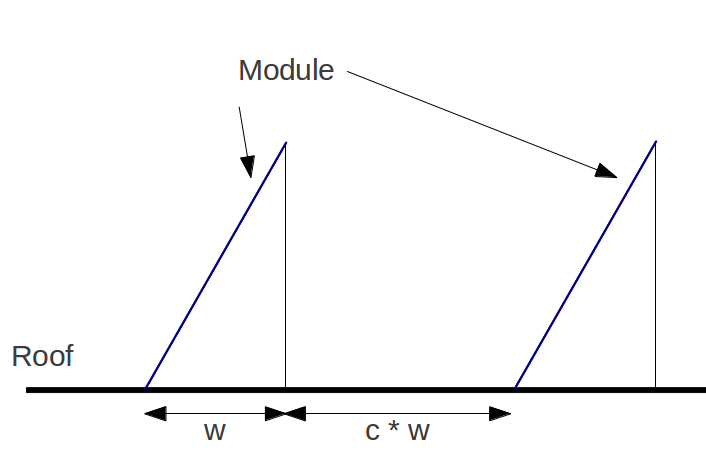
\includegraphics[width=0.5\textwidth]{phase2/group2/figure/flatroofreduction.png}
	\caption{Solar Modules mounted on a mounting system of a flat roof}
	\label{fig:flatroof}
\end{figure}
Furthermore the global irradiance has to be picked from the look-up table. According to Solar Atlas Berlin \citen{solaratlas} areas with a global irradiance less than $905 Wh/m^2$ have to be neglected. Also surface are neglected which have a smaller area then $5m^2$. It is assumed that it is economically not worth the mount modules on such a small roof. The actual calculation of the potential highly depends on the type of module. This will be explained in the following sub sections.



\subsubsection{Potential of Photovoltiac systems}
To calculate the potential of photovoltiac systems two approaches were applied. First the estimation as described by Wagner (2010) \citen{Wagner2010} was implemented. According to Wagner (2010) the energy gain of a photovoltiac system can be calculated with 

\begin{align}
\label{eq:pv_calc}
E &= M \cdot GA \cdot \frac{P}{E_0} \cdot PR \cdot \eta_{EUR} \cdot \eta_l \\\notag\\\notag
\text{with:}&\\\notag
E &:\text{total energy gain per year \(kWh/a\)} \\\notag
E_0 &:\text{1000 \(W/m^2\)} \\\notag
M &:\text{Number of Modules} \\\notag
PR &:\text {Performance ratio} \\\notag
P &:\text{nominal power \(W\)} \\\notag
\eta_{EUR} &:\text{euro inverter efficiency} \\\notag
\eta_l&:\text{transmission efficiency} \\\notag
GA &:\text{Global Irradiation \(kWh/m^2 a\)} \notag
\end{align}

The parameters \(P\),\(\eta_{EUR}\),\(\eta_l\) and \(M\)depend on the photovoltaic cell and the inverter. Values for these parameters are taken from real photovoltiac cells. For the calculations the silicon cell BP 585F from BP Solar \citen{BPSolar} combined with the inverter SP 2500-450 from the company Sun Power \citen{SunPower} has been used. The inverter efficiency is \(\eta_{EUR} = 15 \%\) and the transmission efficiency is set to \(\eta_l = 9\%\). The nominal power of the cell is \(P_0 = 85 W\). This calculation method allows to use real data of photovoltiac cells and considers the inverter.
\\

Because the the Solar Atlas Berlin is the only available reference, finally a second approach according to the Solar Atlas was used. The calculation of the photovoltiac energy is simplified and finally done with equation \ref{eq:pv_calc_SAB}. Where the efficiency coefficient is set to \(e=15\%\) and the system area is the reduced roof surface area.

\begin{align}
\label{eq:pv_calc_SAB}
E &= A \cdot GA \cdot PR \cdot e \\\notag\\\notag
\text{with:}&\\\notag
E &:\text{total energy gain per year \(kWh/a\)} \\\notag
A &:\text{System Area \(m^2\)} \\\notag
e &:\text{efficiency coefficient} \\\notag
GA &:\text{Global Irradiation \(kWh/m^2 a\)} \notag
\end{align}





\subsubsection{Solar Thermal}
The calculation of the potential of solar thermal modules was done as described in Struckmann (2008) \citen{struckmann2008}. According to Struckmann (2008) the useful energy gain $Q_U$ of a solar thermal module is calculated with the formula shown in Equation \ref{eq:st_calc}. Figure \ref{fig:st_module} shows a sketch of a typical solar thermal module and shows the parameter, which are necessary to compute $Q_U$  

\begin{align}
\label{eq:st_calc}
Q_U &= F_R  A \left( I \tau \alpha - U_L \left(T_i - T_a \right) \right)\\\notag\\\notag
\text{with:}&\\\notag
F_R &:\text{ Efficiency Coefficient of the module}\\\notag
A &: \text{ module area, $m^2$}\\\notag
I &: \text{ Solar radiation, $W/m^2$ }\\\notag
\tau &: \text{ transmission coefficient of glazing}\\\notag
\alpha &: \text{ absorption coefficient of plate}\\\notag
U_L &: \text{ collector overall heat loss coefficient, $W/m^2$}\\\notag
T_i &: \text{ input fluid temperature, $^\circ C$}\\\notag
T_a &: \text{ average outside air temperature, $^\circ C$}\notag
\end{align}

\begin{figure}[ht]
	\centering
	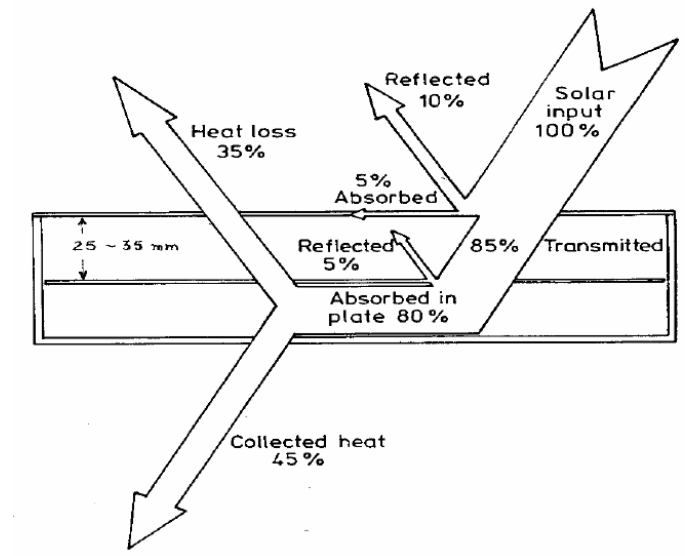
\includegraphics[width=0.5\textwidth]{phase2/group2/figure/st_module.png}
	\caption{typical module with visualization of calculation parameters (Struckmann (2008))}
	\label{fig:st_module}
\end{figure}

For the calculation of the potential a standard solar thermal module has been taken, the TitanPower-AL2DH Flat Plate Collector from the company SunMaxxSolar \citen{sunmaxx}. The efficiency coefficient is assumed to be $F_R = 0.35$ since this value is also used by SimuPLAN for Solar Atlas Berlin. The input fluid temperature is assumed to be $T_i = 10 ^\circ C$ which seems to be a realistic value for the region of Berlin.  Also the average outside air temperature is taken as  $T_a = 10 ^\circ C$.


